\documentclass[11pt,oneside,a4paper]{article}
\usepackage{graphicx}
\usepackage{booktabs}
\usepackage{caption}
\usepackage{subcaption}
\usepackage{amsmath}
\usepackage{amsfonts}
\usepackage{amssymb}
\usepackage{lscape}
\usepackage{psfrag}
\usepackage[usenames]{color}
\usepackage{bbm}
\usepackage[update]{epstopdf}
\usepackage[bookmarks,pdfstartview=FitH,a4paper,pdfborder={0 0 0}]{hyperref}
\usepackage{verbatim}
\usepackage{listings}
\usepackage{textcomp}
\usepackage{fancyhdr}
\usepackage{multirow}
\usepackage{tikz}
\usepackage{lipsum}
\usepackage{xcolor}
\usepackage{wrapfig}
\usepackage[margin=0.5in]{geometry}
\usepackage{pdfpages}
\usepackage[utf8]{inputenc}
\usepackage[compact]{titlesec}
\newcommand{\hint}[1]{{\color{blue} \em #1}}

\makeatletter %% <- make @ usable in command names
\newcommand*\Neg[2][0mu]{\Neginternal{#1}{\negslash}{#2}}
\newcommand*\sNeg[2][0mu]{\Neginternal{#1}{\snegslash}{#2}}
\newcommand*\ssNeg[2][0mu]{\Neginternal{#1}{\ssnegslash}{#2}}
\newcommand*\sssNeg[2][0mu]{\Neginternal{#1}{\sssnegslash}{#2}}
\newcommand*\Neginternal[3]{\mathpalette\Neg@{{#1}{#2}{#3}}}
\newcommand*\Neg@[2]{\Neg@@{#1}#2}
\newcommand*\Neg@@[4]{%
	\mathrel{\ooalign{%
			$\m@th#1#4$\cr
			\hidewidth$\m@th#3{#1}\mkern\muexpr#2*2$\hidewidth\cr
	}}%
}

\newcommand*\negslash[1]{\m@th#1\not\mathrel{\phantom{=}}}
\newcommand*\snegslash[1]{\rotatebox[origin=c]{60}{$\m@th#1-$}}
\newcommand*\ssnegslash[1]{\rotatebox[origin=c]{60}{$\m@th#1{\dabar@}\mkern-7mu{\dabar@}$}}
\newcommand*\sssnegslash[1]{\rotatebox[origin=c]{60}{$\m@th#1\dabar@$}}
\makeatother  %% <- revert @

\makeatletter
\def\cleardoublepage{\clearpage\if@twoside \ifodd\c@page\else%
\hbox{}%
\thispagestyle{empty}%
\clearpage%
\if@twocolumn\hbox{}\clearpage\fi\fi\fi}
\makeatother

\sloppy
% \widowpenalty=10000
% \clubpenalty=10000

\title{
    \vspace*{0.0mm}
    \LARGE\bf\sf Big Data for Engineers (Spring 2020)
    \vspace*{10.0mm} \\
    %
    \Huge\bf\sf Summary
    %
    \vspace*{30.0mm} \\
    \normalsize
    %
    \sf Author:\\[5pt]
    \sf Yannick Merkli\\ [5pt]
    \sf \pageref{lastpage} Pages
}
\date{}

\begin{document}

\maketitle
\thispagestyle{empty}
\raggedbottom
\clearpage

\pagenumbering{roman}

\clearpage
\setcounter{tocdepth}{2}
\tableofcontents
\clearpage
\pagenumbering{arabic}

\setlength\parindent{0pt}
\titlespacing{\subsection}{0pt}{2ex}{2ex}


\newpage

\section{Introduction}

\subsection{History}

Databases have always existed in some way as a way to preserve information. It started with speaking and singing, went on with stone engraving and printing. Even before computers, tables were the primary format to represent data. Things changed drastically with the introduction of computers. Database management systems (DBMS) started with file systems (1960s), then we entered the relational era (1970s) and finally progressed into the NoSQL era (2000s) with the upcoming of big data.

\subsection{Big Data}

Big Data is a buzzword that goes across many disciplines (distributed systems, high-performance computing, data management, algorithms, statistics, machine learning, etc.) and that involves a lot of proprietary technology (AWS, Google Cloud, Microsoft Azure, etc.) which is simply a result of the need of companies to have efficient data systems.

The big in big data: \textbf{three Vs}

\vspace{-\topsep}
\begin{itemize}
	\setlength{\itemsep}{0pt}
	\setlength{\parskip}{0pt}
	\item Volume: Nowadays we have lots of sources of data (web, sensors, proprietary, scientific). Storage has become so cheap that we often just store data because we can. Further, data carries value; data is worth more than the sum of its parts (data totality: one must have complete data).
	\item Variety: We have different \textbf{data shapes}: tables, trees, graphs, cubes, text.
	\item Velocity: Data is generated automatically, Data is a realtime byproduct of human activity
\end{itemize}

\textbf{Prefixes (International System of Units)}

\begin{tabular}{|c|r|c|r|}
	\hline 
	kilo (k) & 1,000 (3 zeros) & kibi (ki) & 1,024 ($2^{10}$) \\ 
	\hline 
	Mega (M) & 1,000,000 (6 zeros) & Mebi (Mi) & 1,048,576 ($2^{20}$) \\ 
	\hline 
	Giga (G) & 1,000,000,000 (9 zeros) & Gibi (Gi) & 1,073,741,824 ($2^{30}$) \\ 
	\hline 
	Tera (T) & 1,000,000,000,000 (12 zeros) & Tebi (Ti) & 1,099,511,627,776 ($2^{40}$) \\ 
	\hline 
	Peta (P) & 1,000,000,000,000,000 (15 zeros) & Pebi (Pi) & 1,125,899,906,842,624 ($2^{50}$) \\ 
	\hline 
	Exa (E) & 1,000,000,000,000,000,000 (18 zeros) & Exbi (Ei) & 1,152,921,504,606,846,976 ($2^{60}$) \\ 
	\hline 
	Zetta (Z) & 1,000,000,000,000,000,000,000 (21 zeros) & Zebi (Zi) & 1,180,591,620,717,411,303,424 ($2^{70}$) \\ 
	\hline 
	Yotta (Y) & 1,000,000,000,000,000,000,000,000 (24 zeros) & Yobi (Yi) & 1,208,925,819,614,629,174,706,176 ($2^{80}$) \\ 
	\hline
\end{tabular}\newline

There are three paramount factors to big data:

\vspace{-\topsep}
\begin{itemize}
	\setlength{\itemsep}{0pt}
	\setlength{\parskip}{0pt}
	\item Capacity: "How much data can we store?"
	\item Throughput: "How fast can we transmit data?"
	\item Latency: "When do I start receiving data?"
\end{itemize}
\vspace{-\topsep}

Capacity has improved incredibly much over the past 60 years (1956: huge HDD had 5MB storage, 2020: there are palm sized 20TB HDDs). Capacity has increased by a factor $200 * 10^9$ (per unit of volume). However, throughput and latency have only improved by a factor $10'000$ and $200$ respectively. This discrepancy creates problems: the throughput no longer scales to the amount of data and the latency no longer scales to the throughput. Solution:

\vspace{-\topsep}
\begin{itemize}
	\setlength{\itemsep}{0pt}
	\setlength{\parskip}{0pt}
	\item Capacity-throughput discrepancy: parallelization
	\item Throughput-latency discrepancy: batch processing
\end{itemize}
\vspace{-\topsep}

\textbf{What is big data?}

Big Data is a portfolio of technologies that were designed to store, manage and analyze data that is too large to fit on a single machine while accommodating for the issue of growing discrepancy between
capacity, throughput and latency.

\section{Lessons learnt from the past}

\textbf{Data Independence:}\\
An underlying principle that has been valid for a long time is the principle of \textbf{data independence} (developed by Edgar Codd): Data Independence is defined as a property of DBMS that helps you to change the Database schema at one level of a database system without requiring to change the schema at the next higher level. Data independence helps you to keep data separated from all programs that make use of it.\\
This means we could e.g. change the physical storage (e.g. iPad instead of HDD) \textit{without} changing the logical data model.\\

\textbf{Overall architecture}\\
The overall architecture of a DBMS consists of:

\vspace{-\topsep}
\begin{itemize}
	\setlength{\itemsep}{0pt}
	\setlength{\parskip}{0pt}
	\item Language (e.g. SQL)
	\item Model (e.g. Tables (old); graphs, trees, cubes (new)
	\item Compute (e.g. single CPU (old); hadoop cluster (new))
	\item Storage (e.g. HDD (old); distributed storage (new)
\end{itemize}
\vspace{-\topsep}

A data model essentially describes \textit{what data looks like} and \textit{what you can do with the data}.

\subsection{Basic concepts}

\begin{itemize}
	\setlength{\itemsep}{0pt}
	\setlength{\parskip}{0pt}
	\item Table (Collection): A set of rows (= business object, item, entity, document, record) and each row has attributes (= columns)
	\item Attribute (column, field, property): A certain attribute of a row
	\item Primary key (row ID, name): a unique identifier of a row
\end{itemize}
\vspace{-\topsep}

\subsection{Relational Algebra}

We can look at tables as relations or as partial functions, mapping property to value\\
($f \in \mathbb{S} \ssNeg \rightarrow \mathbb{V}$), e.g. $city \mapsto Zurich$.

\subsubsection{Relations (the math, for database scientists)}

A relation R is made of:
\vspace{-\topsep}
\begin{itemize}
	\setlength{\itemsep}{0pt}
	\setlength{\parskip}{0pt}
	\item A set of attributes: $Attributes_R \subseteq \mathbb{S}$
	\item An extension (set of tuples): $$Extension_R \subseteq \mathbb{S} \ssNeg \rightarrow \mathbb{V} \quad s.t. \quad \forall t \in Extension_R, support(t) = Attributes_R$$
\end{itemize}
\vspace{-\topsep}

\textbf{Tabular integrity:} Holds if all rows have the same attributes and have a valid value for the attributes.\\
\textbf{Atomic integrity:} No tables in tables.\\
\textbf{Domain integrity:} All attribute values are of the specified type (e.g. an attribute \textit{Name} of type string can't be an integer).\\

In SQL, tabular integrity, atomic integrity and domain integrity all hold. In NoSQL however, none of these three properties hold.

\subsection{Relational queries}

The following table shows the operators used in Relational Algebra.

\vspace{-\topsep}
\begin{figure}[hb]
	\centering
	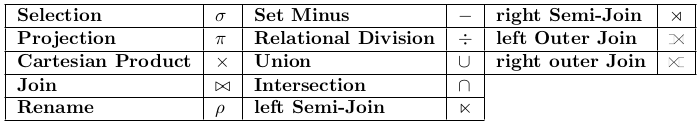
\includegraphics[width=0.7\linewidth]{figures/relational_algebra_operators}
	\label{fig:relationalalgebraoperators}
\end{figure}
\vspace{-\topsep}

\textbf{Projection:} The projection operator is used to produce from a relation R a new relation that has only some of R’s columns. The value of expression $\prod_{A_1,...,A_n}(R)$ is a relation that only
consists of columns for the attributes $A_1,...,A_n$.

\textbf{Selection:} The selection operator applied to R produces a new relation with a subset of R’s tuples, namely those who meet some condition C. This operation is denoted by $\sigma_C(R)$.

\textbf{Cartesian product:} The Cartesian product of relations R, S, denoted $R \times S$, simply concatenates every possible combination of tuples $r \in R, s \in S$. If R, S have attributes in common: rename them. In practice rarely used without join operators.

\textbf{Natural Join:} The natural join of relations L, R, denoted $L \bowtie R$, pairs only those tuples from L and R that agree in whatever attributes they share commonly. Natural Join is associative!
Other variants:

\vspace{-\topsep}
\begin{itemize}
	\setlength{\itemsep}{0pt}
	\setlength{\parskip}{0pt}
	\item Left outer join: natural join \& unmatched tuples from L
	\item Right outer join: natural join \& unmatched tuples from R
	\item Full outer join: natural join \& unmatched tuples from both L and R
	\item Left semi join: tuples from L that match with some tuple in R
	\item Right semi join: tuples from R that match with some tuple in L
\end{itemize}
\vspace{-\topsep}

\textbf{Theta-Join:} A theta join $\bowtie_\theta$ allows to join tuples from two relations R, S based on an arbitrary condition $\theta$ rather than solely based on attribute agreement. We get this new relation by:

\vspace{-\topsep}
\begin{enumerate}
	\setlength{\itemsep}{0pt}
	\setlength{\parskip}{0pt}
	\item Take the Cartesian product $R \times S$
	\item select those tuples satisfying condition $\theta$
\end{enumerate}
\vspace{-\topsep}

\textbf{Union, Intersection, Set Minus:} requires: both relations have the same schema $\rightarrow$ then consider set of tuples, do corresponding set operations. Note that $R \cap S = R - (R - S)$

\textbf{Rename:} 

\vspace{-\topsep}
\begin{itemize}
	\setlength{\itemsep}{0pt}
	\setlength{\parskip}{0pt}
	\item to change the name of the relation R to S, we write $\rho_S(R)$. 
	\item to rename attributes of R, we use the operator $\rho_{(A_1,..,A_n)}(R)$ where the attributes in the result relation S are called $A_1,...,A_n$, respectively.
\end{itemize}
\vspace{-\topsep}

\subsection{Terminology}

Data: Data Manipulation Language (DML) (Query, insert, remove rows)
Schema: Data Definition Language (DDL) (Create or table/schema, drop it)
\vspace{-\topsep}
\begin{figure}[hb]
	\centering
	\begin{subfigure}[t]{.5\textwidth}
		\centering
		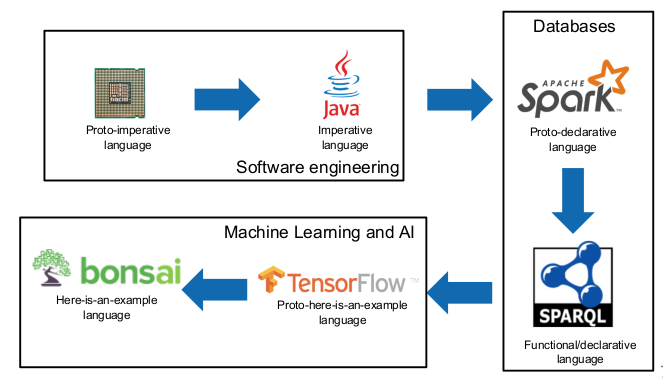
\includegraphics[width=0.8\linewidth]{figures/language_landscape}
		\caption{Language landscape}
		\label{fig:languagelandscape}
	\end{subfigure}%
	\begin{subfigure}[t]{.5\textwidth}
		\centering
		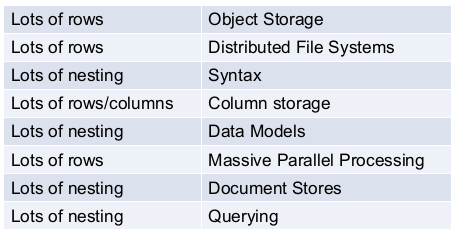
\includegraphics[width=0.8\linewidth]{figures/scaling_up_overview}
		\caption{Data Scale-Up}
		\label{fig:scalingupoverview}
	\end{subfigure}
\end{figure}
\vspace{-\topsep}

\subsection{Transactions}

The good old times of databases: ACID (Atomicity, Consistency, Isolation, Durability).

\vspace{-\topsep}
\begin{itemize}
	\setlength{\itemsep}{0pt}
	\setlength{\parskip}{0pt}
	\item Atomicity: Either the entire transaction is applied, or none of it (rollback).
	\item Consistency: After a transaction, the database is in a consistent state again.
	\item Isolation: A transaction feels like nobody else is writing to the database.
	\item Durability: Updates made do not disappear again.
\end{itemize}
\vspace{-\topsep}

\subsection{Performance}

Optimize for read vs. write intensive:
\vspace{-\topsep}
\begin{itemize}
	\setlength{\itemsep}{0pt}
	\setlength{\parskip}{0pt}
	\item OnLine Transaction Processing	(OLTP):	Write-intensive
	\item OnLine Analytical Processing (OLAP): Read-intensive
\end{itemize}

There is no such thing as "one size fits all" - data shape matters.

\subsection{Data scale-up}

Data can have lots of rows, lots of columns and lots of nesting. For the rest of this lecture, we are concerned with exactly this: scaling up!

\newpage

\titlespacing{\subsection}{0pt}{0ex}{0ex}

\section{SQL}

SQL is a family of standards, namely it includes a data definition language for schemas, a data manipulation language for updates and a query language for reads. Note that SQL is case-insensitive.

\subsection{DDL: Data Definition Language}
\vspace{-\topsep}
\begin{figure}[hb!]
	\centering
	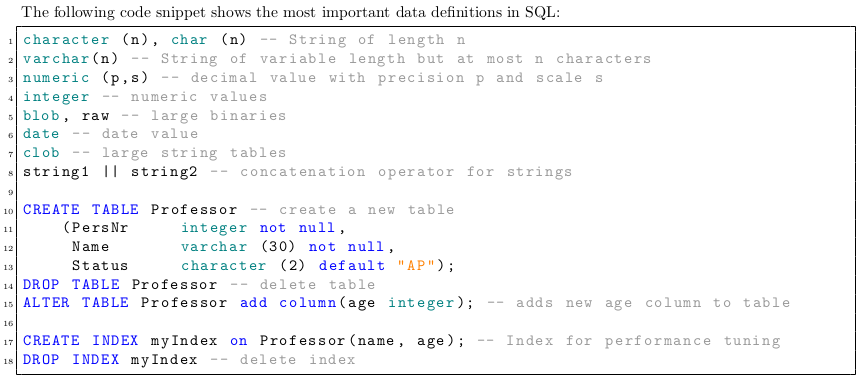
\includegraphics[width=1\linewidth]{figures/sql_1}
	\label{fig:sql1}
\end{figure}
\vspace{-\topsep}

\subsection{DML: Data Manipulation Language}
\vspace{-\topsep}
\begin{figure}[hb!]
	\centering
	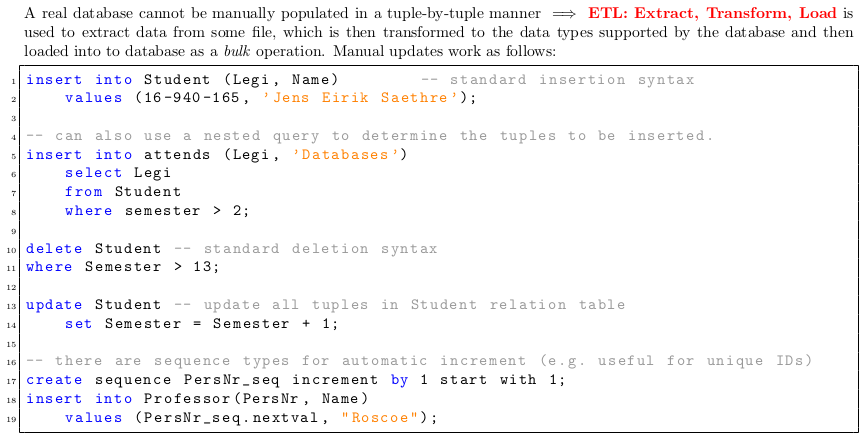
\includegraphics[width=1\linewidth]{figures/sql_2}
	\label{fig:sql2}
\end{figure}
\vspace{-\topsep}

\subsection{Simple Queries in SQL}
\vspace{-\topsep}
\begin{figure}[hb!]
	\centering
	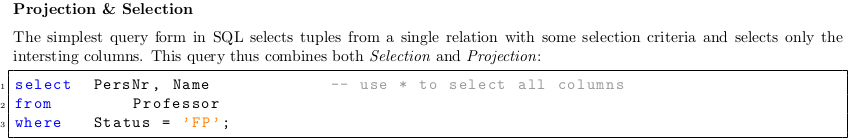
\includegraphics[width=1\linewidth]{figures/sql_3}
	\label{fig:sql3}
\end{figure}
\vspace{-\topsep}

\newpage
\vspace{-\topsep}
\begin{figure}[t!]
	\centering
	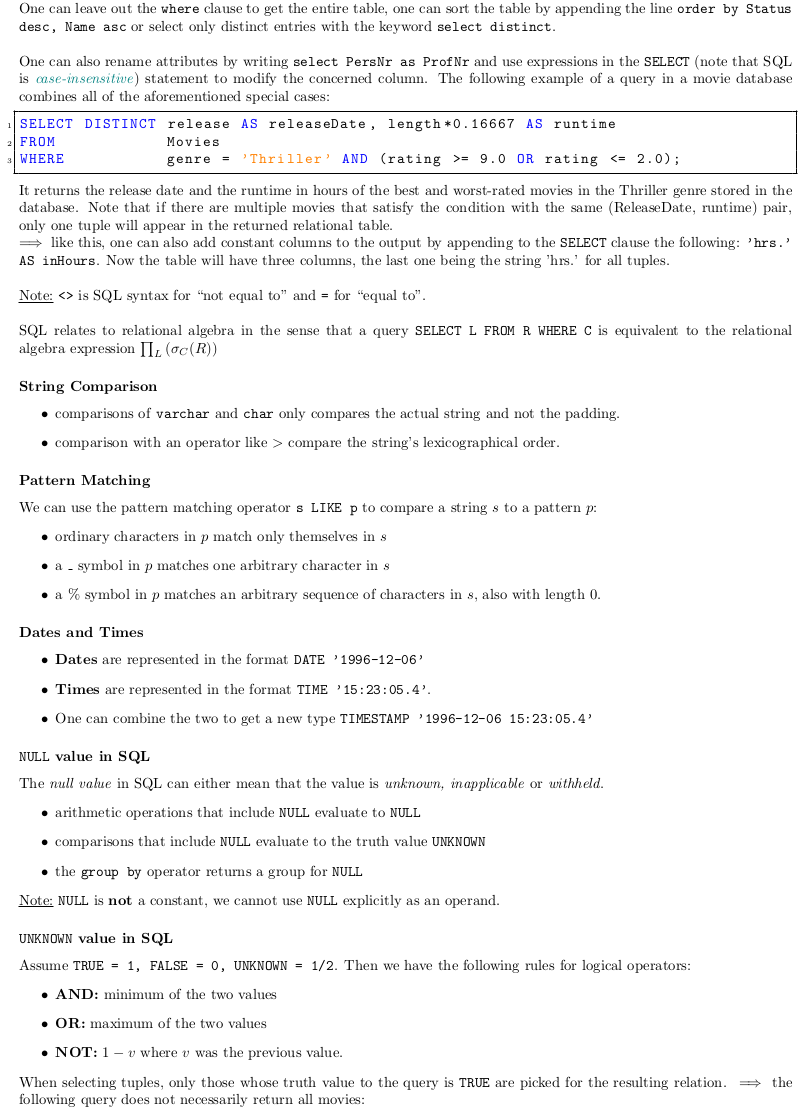
\includegraphics[width=1\linewidth]{figures/sql_4}
	\label{fig:sql4}
\end{figure}
\vspace{-\topsep}

\newpage

\vspace{-\topsep}
\begin{figure}[t!]
	\centering
	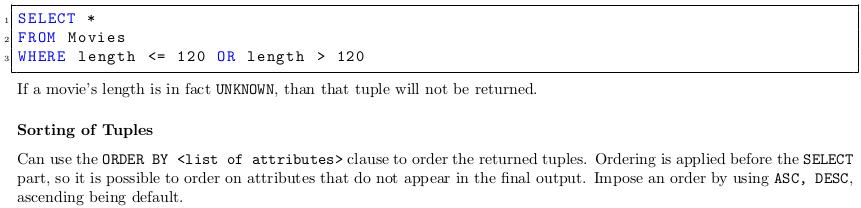
\includegraphics[width=0.95\linewidth]{figures/sql_5}
	\label{fig:sql5}
\end{figure}
\vspace{-\topsep}

\subsection{Queries on multiple Relations}

\vspace{-\topsep}
\begin{figure}[hb!]
	\centering
	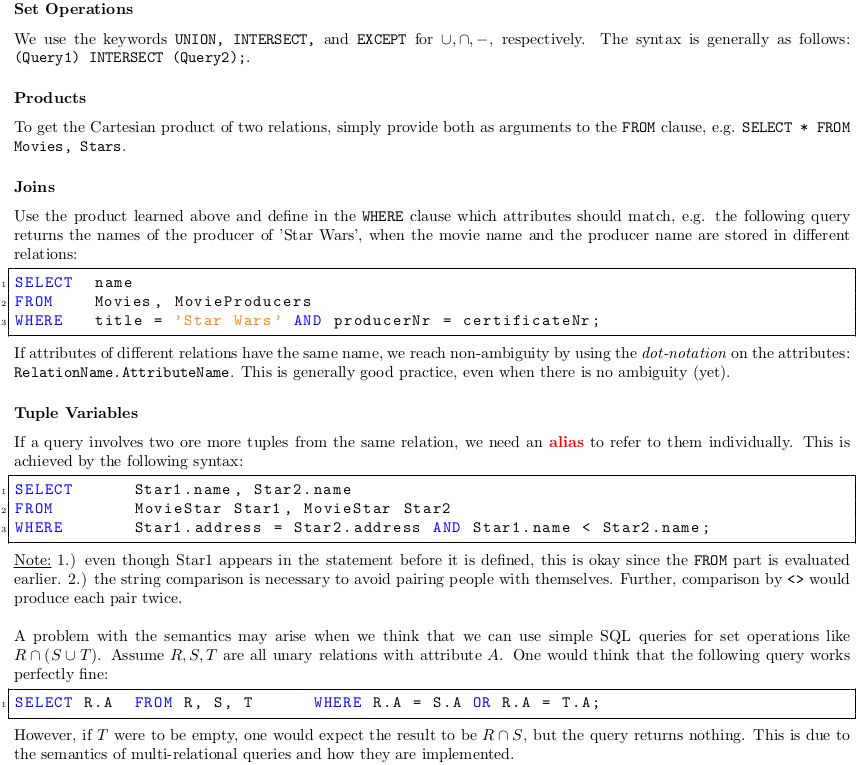
\includegraphics[width=1\linewidth]{figures/sql_6}
	\label{fig:sql6}
\end{figure}
\vspace{-\topsep}

\subsection{Full-Relation Operations}
\vspace{-\topsep}
\begin{figure}[hb!]
	\centering
	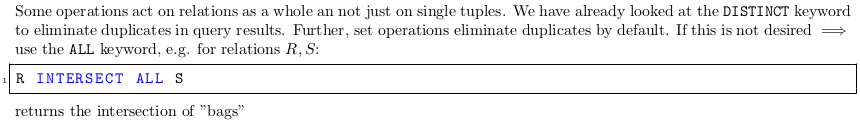
\includegraphics[width=1\linewidth]{figures/sql_7}
	\label{fig:sql7}
\end{figure}
\vspace{-\topsep}

\newpage

\vspace{-\topsep}
\begin{figure}[hb!]
	\centering
	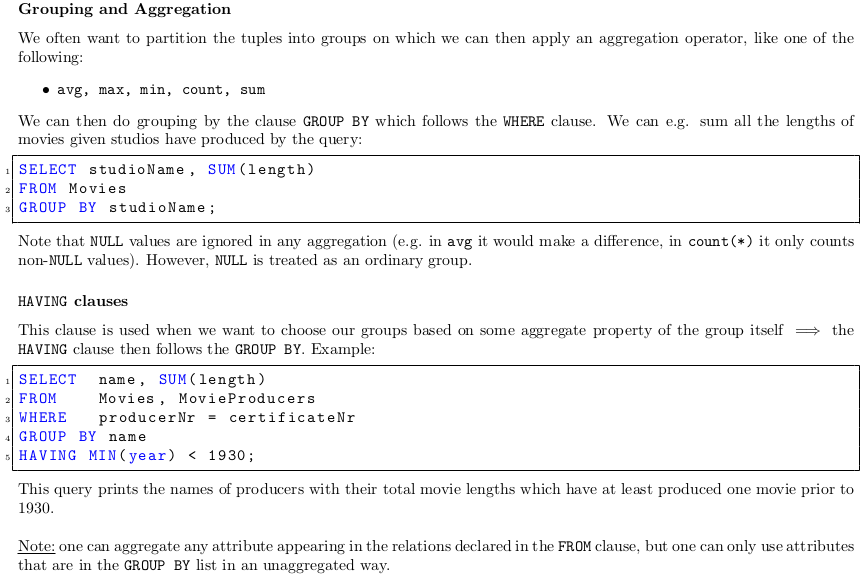
\includegraphics[width=1\linewidth]{figures/sql_8}
	\label{fig:sql8}
\end{figure}
\vspace{-\topsep}

\subsection{Subqueries}

\vspace{-\topsep}
\begin{figure}[hb!]
	\centering
	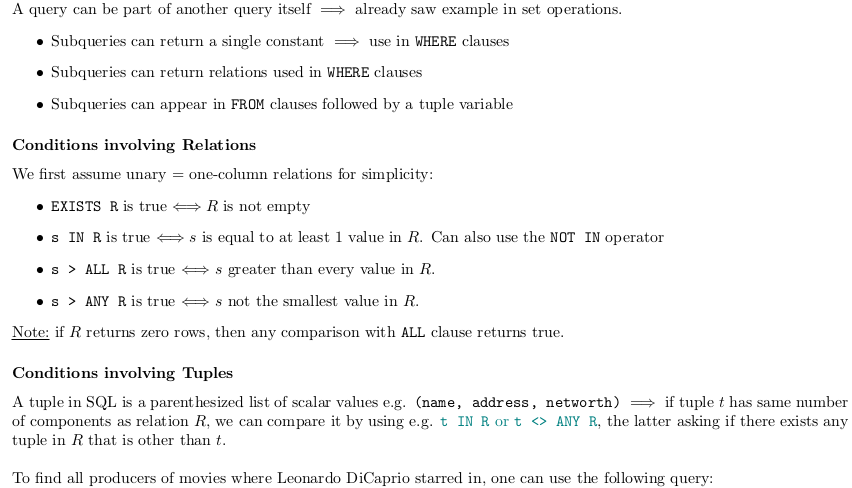
\includegraphics[width=1\linewidth]{figures/sql_9}
	\label{fig:sql9}
\end{figure}
\vspace{-\topsep}

\newpage

\vspace{-\topsep}
\begin{figure}[hb!]
	\centering
	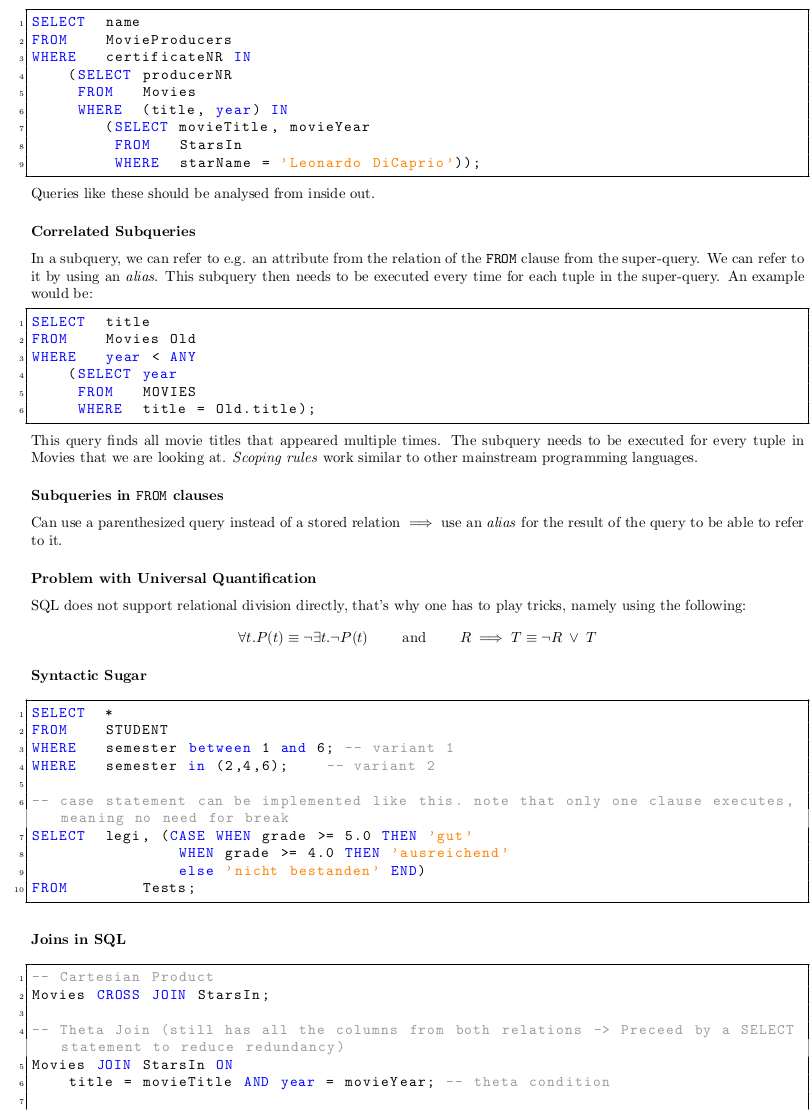
\includegraphics[width=1\linewidth]{figures/sql_10}
	\label{fig:sql10}
\end{figure}
\vspace{-\topsep}

\newpage

\vspace{-\topsep}
\begin{figure}[hb!]
	\centering
	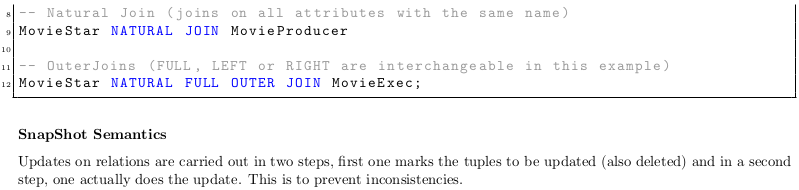
\includegraphics[width=1\linewidth]{figures/sql_11}
	\label{fig:sql11}
\end{figure}
\vspace{-\topsep}

\subsection{Views}

\vspace{-\topsep}
\begin{figure}[hb!]
	\centering
	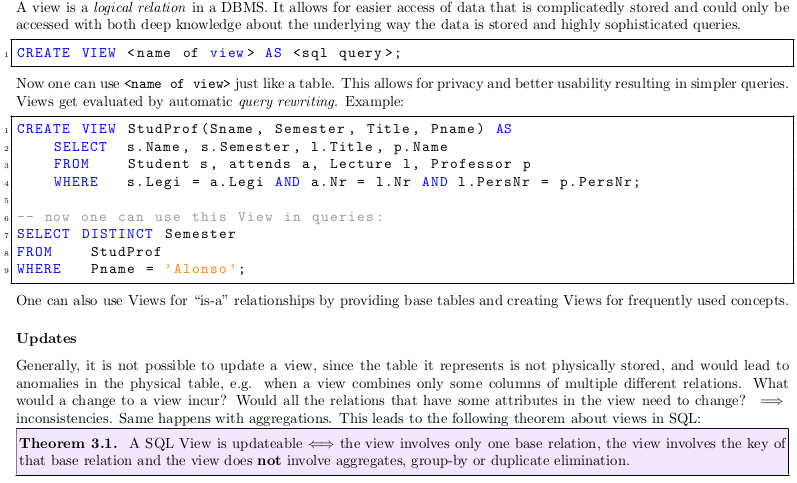
\includegraphics[width=1\linewidth]{figures/sql_12}
	\label{fig:sql12}
\end{figure}
\vspace{-\topsep}

\titlespacing{\subsection}{0pt}{2ex}{2ex}



\label{lastpage} % this must stay here
\clearpage
\addcontentsline{toc}{section}{References}
\bibliographystyle{acm}
\bibliography{refs}

\clearpage
\appendix
\pagenumbering{Roman}

\end{document}
